\section{Экономически-организационная часть}
\subsection{Введение}
Экономическая часть посвящена разработке комплекса мероприятий организационно–экономического и финансового планов, которые необходимо выполнить для создания программного продукта, позволяющего проводить анализ и моделирование производительности программ.

Система разработана на языке программирования Python, и включает в себя группу проектов анализа данных в системе проведения статистических исследований Orange. Программный продукт не может быть интегрирован в другие программные комплексы и предназначен для внутреннего использования. Заказчиком является структурное подразделение МГТУ им. Н. Э. Баумана.
Данный проект не преследует цель получения прибыли.

\subsection{Основные этапы проекта разработки нового изделия}
Основные этапы проекта разработки нового изделия представлены в таблице \ref{tab:development-stages}.

\begin{table}[H]
    \caption{\label{tab:development-stages}Основные этапы разработки проекта}
    \begin{tabular}[H]{|l|p{5cm}|p{8cm}|}
        \hline
        № & Условное обозначение & Описание\\
        \hline
        1 & Техническое задание (ТЗ) & Предпроектное обследование. Постановка задачи по созданию программного продукта\\
        \hline
        2 & Эскизный проект (ЭП) & Проработка использования основных технологий и инструментов, необходимых для выполнения программного продукта\\
        \hline
        3 & Технорабочий проект (ТП) & Разработка модели анализа: структуры данных и реализации алгоритмов анализа. Разработка программного решения\\
        \hline
        4 & Документация и внедрение (В) & Подготовка и передача программного продукта и программной документации\\
        \hline
    \end{tabular}
\end{table}

\subsection{Расчёт трудоёмкости разработки программного продукта}
Трудоёмкость разработки программного продукта рассчитывается по формуле
\begin{equation*}
	\tau_{\pe\pe} = \tau_{\te\ze} + \tau_{\erev\pe} + \tau_{\te\pe} + \tau_{\re\pe} + \tau_{\ve},
\end{equation*}
где $\tau_{\te\ze}$ -- трудоёмкость разработки технического задания на создание ПП; $\tau_{\erev\pe}$ -- трудоёмкость разработки эскизного проекта ПП; $\tau_{\re\pe}$ -- трудоёмкость разработки рабочего проекта ПП; $\tau_{\ve}$ -- трудоёмкость внедрения разработанного ПП.

Трудоёмкость разработки технического задания можно рассчитать по формуле
\begin{equation*}
	\tau_{\te\ze} = T_{\ze\re\ze} + T_{\ze\re\pe}
\end{equation*}
где $T_{\ze\re\ze}$ -- затраты времени разработчика постановки задачи на разработку ТЗ, человеко-дни, $T_{\ze\re\pe}$ -- затраты времени разработчика программного обеспечения на разработку ТЗ, человеко-дни.

Значения затрат времени $T_{\ze\re\ze}$ и $T_{\ze\re\pe}$ определяют по формулам:
\begin{eqnarray*}
	T_{\ze\re\ze} = t_{\ze} K_{\ze\re\ze} \\
	T_{\ze\re\pe} = t_{\ze} K_{\ze\re\pe},
\end{eqnarray*}
где $t_{\ze}$ -- норма времени на разработку ТЗ на программный продукт в зависимости от функционального назначения и степени новизны разрабатываемого ПП, человеко-дни;

$K_{\ze\re\ze}$ -- коэффициент, учитывающий удельный вес трудоемкости работ, выполняемых разработчиком постановки задач на стадии ТЗ (в случае совместной с разработчиком ПО разработки $K_{\ze\re\ze}=0,65$, в случае самостоятельной разработки ТЗ $K_{\ze\re\ze}=1$); 
$K_{\ze\re\pe}$ -- коэффициент, учитывающий удельный вес трудоемкости работ, выполняемых разработчиком ПП на стадии ТЗ (в случае совместной с постановки задач разработки $K_{\ze\re\pe} = 0,35$, в случае самостоятельной разработки ТЗ $K_{\ze\re\pe} = 1$).

В данном случае следует принять следующие значения коэффициентов
\begin{equation}
	t_{\ze} = 3 \che\e\el.-\de\en\e\ishrt.
\end{equation}

Тогда трудоёмкость разработки технического задания
\begin{equation}
	\tau_{\te\ze} = T_{\ze\re\ze} + T_{\te\re\pe} = 3 \cdot 1 = 3 \che\e\el.-\de\en\e\ishrt.
\end{equation}

Трудоёмкость разработки эскизного проекта ПП рассчитывают по формуле
\begin{equation}
	\tau_{\erev\pe} = T_{\erev\re\ze} + T_{\erev\re\pe},
\end{equation}
где $T_{\erev\re\ze}$ -- затраты времени разработчика постановки задачи на разработку эскизного проекта, человеко-дни, $T_{\erev\re\pe}$ -- затраты времени разработчика ПП на разработку эскизного проекта, человеко-дни.

Значения величин $T_{\erev\re\ze}$ и $T_{\erev\re\pe}$ рассчтываются по формулам:
\begin{eqnarray*}
	T_{\erev\re\pe} = t_{\erev} K_{\erev\re\pe}
	T_{\erev\re\ze} = t_{\erev} K_{\erev\re\ze}, \\
\end{eqnarray*}

где $t_{erev}$ -- норма времени на разработку эскизного проекта на ПП в зависимости от функционального назначения и степени новизны разрабатываемого ПП, человеко-дни;

$K_{\erev\re\pe}$ -- коэффициент, учитывающий удельный вес трудоёмкости работ, выполняемых разработчиком постановки задач на стадии эскизного проекта;

$K_{\erev\re\ze}$ -- коэффициент, учитывающий удельный вес трудоёмкости работ, выполняемых разработчиком ПП на стадии эскизного проекта.

В данном случае следует принять следующие значения коэффициентов
\begin{equation*}
	t_{\erev} = 18 \che\e\el.-\de\en\e\ishrt, K_{\erev\re\pe} = 0, K_{\erev\re\ze} = 1.
\end{equation*}
Тогда трудоемкость разработки эскизного проекта ПП равна
\begin{equation*}
	\tau_{\erev\pe} = T_{\erev\re\ze} + T_{\erev\re\pe} = 18 \che\e\el.-\de\en\e\ishrt.
\end{equation*}

Трудоемкость разработки технического проекта зависит от функционального назначения ПП, количества разновидностей форм входной и выходной информации и определяется как сумма времени, затраченного разработчиком постановки задач и разработчиком программного обеспечения: 
\begin{equation*}
	\tau_{\te\pe} = (t_{\te\re\ze} + t_{\te\re\pe}) \cdot K_{\ve} K_{\re},
\end{equation*}
где $t_{\te\re\ze}$ и $t_{\te\re\pe}$ -- норма времени, затрачиваемого на разработку ТП разработчиком постановки задач и разработчиком ПП соответственно, человеко-дни ($t_{\te\re\pe} = 20\che\e\el.-\de\en\e\ishrt$);

$K_{\ve}$ -- коэффициент учёта вида используемой информации;

$K_{\re}$ -- коэффициент учёта режима обработки информации ($K_{\re} = 1,26$).

Значение коэффициента $K_{\ve}$ определяется по формуле
\begin{equation*}
    K_{\ve} = \frac{K_{\pe}n_{\pe} + K_{\en\es}n_{\en\es} + K_{\be}n_{\be}}{n_{\pe} + n_{\en\es} + n_{\be}}
\end{equation*}
 
где	$K_{\pe}$, $K_{\en\es}$, $K_{\be}$, -- значения коэффициентов учета вида используемой информации для переменной, нормативно–справочной информации и баз данных соответственно;
$n_{\pe}$, $n_{\en\es}$, $n_{\be}$ -- количество наборов данных переменной, нормативно–справочной информации и баз данных соответственно. 
\begin{equation*}
	K_{\ve} = (1,0\cdot4 + 0,72\cdot2 + 2,08\cdot4)/10 = 1,376
\end{equation*}
Тогда трудоемкость разработки технического проекта
\begin{equation*}
	\tau_{\te\pe} = (t_{\te\re\ze} + t_{\te\re\pe}) \cdot K_{\ve} K_{\re} = 20 \cdot 1,26 \cdot 1,376 = 35 \che\e\el.-\de\en\e\ishrt,
\end{equation*}
Трудоемкость разработки рабочего проекта зависит от функционального назначения ПП, количества разновидностей форм входной и выходной информации, сложности алгоритма, сложности контроля информации, степени использования готовых программных модулей, уровня алгоритмического языка программирования и определяется по формуле:
\begin{equation*}
	\tau_{\re\pe} = (t_{\re\re\ze} + t_{\re\re\pe}) \cdot K_{\ka} K_{\re} K_{\ya} K_{\ge} K_{\ci\ca},
\end{equation*}
где $K_{\ka}$ -- коэффициент учета сложности контроля информации ($K_{\ka} = 1,00$);
$K_{\re}$ -- коэффициент учета режима обработки информации ($K_{\re} = 1,32$); 
$K_{\ya}$ -- коэффициент учета уровня используемого алгоритмического языка программирования ($K_{\ya} = 1,00$); 
$K_{\ge}$ -- коэффициент учета степени использования готовых программных модулей -- 25\% – 40\% ($K_{\ge} = 0,70$); 
$K_{\ci\ca}$ -- коэффициент учета вида используемой информации и сложности алгоритма ПП.
Значение коэффициента $K_{\ci\ca}$ определяют по формуле
\begin{equation*}
    K_{\ci\ca} = \frac{K'_{\pe}n_{\pe} + K'_{\en\es}n_{\en\es} + K'_{\be}n_{\be}}{n_{\pe} + n_{\en\es} + n_{\be}}
\end{equation*}
где $K'_{\pe}$, $K'_{\en\es}$, $K'_{\be}$ -- значения коэффициентов учета сложности алгоритма ПП и вида используемой информации для переменной, нормативно–справочной информации и баз данных соответственно, $K_{\ci\ca} = 0,98$;
$t_{\re\re\ze}$, $t_{\re\re\pe}$ -- норма времени, затраченного на разработку РП на алгоритмическом языке высокого уровня разработчиком постановки задач и разработчиком программного обеспечения соответственно, чел.–дни. ($t_{\re\re\pe} = 51$ чел.-дней), так как используется 2 вида входной и 2 вида выходной информации.
 
Соответственно трудоемкость технорабочего проекта можно рассчитать следующим образом:
\begin{equation*}
	\tau_{\te\re\pe}=0,85 \cdot \tau_{\te\pe} + \tau_{\re\pe} = 0,85 \cdot 35 + 50 = 80 \che\e\el.-\de\en\e\ishrt.
\end{equation*}
Трудоемкость выполнения стадии внедрения рассчитывается по формуле:
\begin{equation*}
	t_{\ve} = (t_{\ve\re\ze} + t_{\ve\re\pe}) \cdot K_{\ka} K_{\re} K_{\ze},
\end{equation*}
где $t_{\ve\re\ze}$, $t_{\ve\re\pe}$ -- норма времени, затрачиваемого разработчиком постановки задач и разработчиком программного обеспечения соответственно на выполнение процедур внедрения ПП, человеко–дни. 
\begin{eqnarray*}
	t_{\ve\re\pe} = 10 \che\e\el.-\de\en\e\ishrt, \\
	K_{\ka} = 1,08, K_{\re} = 1,32, K_{\ze} = 0,7.
\end{eqnarray*}
Подставив значения коэффициентов, получим
\begin{equation*}
	t_{\ve} = (t_{\ve\re\ze} + t_{\ve\re\pe}) \cdot K_{\ka} K_{\re} K_{\ze} = 10\cdot1,08\cdot1,32\cdot0,7 \approx 10 \che\e\el.-\de\en\e\ishrt.
\end{equation*}
Таким образом, трудоемкость разработки программной продукции   составляет
\begin{equation*}
	\tau_{\pe\pe} = 3 + 18 + 80 + 10 = 111 \che\e\el.-\de\en\e\ishrt.
\end{equation*}
Планирование и контроль хода выполнения разработки проводят по календарному графику выполнения работ. Можно использовать ленточный график (график Гантта), который представляет собой графическое отображение выполненной работы и времени, затраченного на эту работу, т. е. продолжительность выполнения данной работы.
Продолжительность выполнения всех работ по этапам разработки ПП определяют из выражения
\begin{equation*}
	T_i = \frac{(t_i + Q)}{n_i \cdot f},
\end{equation*}
где $t_i$ -- трудоемкость i-й работы, чел.–дни; 
$Q$ -- трудоемкость дополнительных работ, выполняемых исполнителем, чел-дни; 
$n_i$ -- количество исполнителей, выполняющих i-ю работу, чел;
$f$ -- коэффициент пересчета из рб.–дн. в кл.–дн., равный, для 2013 года, 248/365=0,679.

\begin{table}[H]
    \caption{\label{tab:development-stages-calc}Расчёт основных этапов разработки проекта}
    \begin{tabular}[H]{|l|l|l|l|l|}
        \hline
        этап & $t_i$, чел.-дн. & кол-во исполнителей & рб.-дн. & кл-дн.\\
        \hline
        ТЗ & 3 & 1 & 3 & 4\\
        \hline
        ЭП & 18 & 1 & 18 & 26\\
        \hline
        ТРП & 80 & 1 & 80 & 112\\
        \hline
        В & 10 & 1 & 10 & 15\\
        \hline
        Всего &  &  &  111 & 157\\
        \hline
    \end{tabular}
\end{table}

\subsection{Календарный план-график проекта}
Для иллюстрации последовательности проводимых работ проекта применяют ленточный график, календарный план–график, диаграмму Гантта. На диаграмме Гантта на оси Х показывают календарные дни (по рабочим неделям) от начала проекта до его завершения. По оси Y – выполняемые этапы работ.

Для наглядности приведём график Гантта отражающий взаимодействие шагов проекта во времени. График показывает последовательность действий в нужном порядке и те из них, которые могут выполняться одновременно.
\begin{figure}[H]
    \center{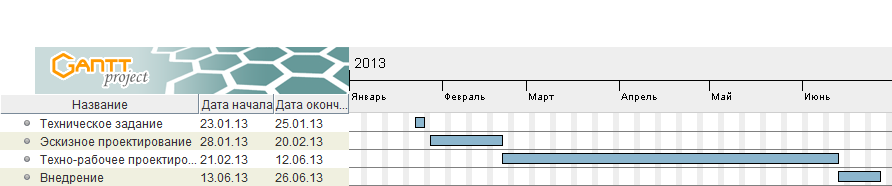
\includegraphics[width=1\linewidth]{Gantt}}
    \caption{Диаграмма Гантта.}
    \label{img:gantt}
\end{figure}

\subsection{Затраты на разработку программного продукта}
Затраты на разработку программной продукции могут быть представлены в виде сметы затрат, включающей в себя следующие статьи:
\begin{itemize}
	\item материальные затраты;
	\item амортизационные отчисления;
	\item расчёт заработной платы;
	\item отчисления в фонды;
	\item прочие затраты.
\end{itemize}

\subsubsection{Расчёт материальных затрат}
Суммарные затраты на материалы состоят из стоимости материалов и транспортно-заготовительных расходов, т.е. 
\begin{equation*}
    C_{\cm} = K_{\te\pe} \sum_{i} \CE_i V_i,
\end{equation*}
где $K_{\te\pe}$ -- коэффициент транспортно-заготовительных расходов ($K_{\te\pe} = 0,19$);

$\CE_i$ -- цена единицы i-го материала, руб.;

$V_i$ -- приобретённое количество i-го материала, шт.

\begin{table}[H]
    \caption{\label{tab:materials}Расходы на материалы}
    \begin{tabular}[H]{|l|l|l|l|l|}
        \hline
        \specialcell{Наименование\\материала} & \specialcell{Единица\\измерения} & Количество & \specialcell{Цена\\единицы, руб.} & Сумма, руб.\\
        \hline
        Диск DVD+R & шт. & 2 & 30 & 60\\
        \hline
        Устройство флэш-памяти & шт. & 1 & 800 & 800\\
        \hline
        Итого &  &  &  & 860\\
        \hline
    \end{tabular}
\end{table}

\subsubsection{Расчёт затрат на оборудование}

Расчёт ведётся по той же формуле, что и для материальных затрат.

\begin{table}[H]
    \caption{\label{tab:devices}Расходы на оборудование}
    \begin{tabular}[H]{|l|l|l|l|l|}
        \hline
        \specialcell{Наименование\\оборудования} & \specialcell{Единица\\измерения} & Кол-во & \specialcell{Цена\\ед., руб.} & \specialcell{Сумма,\\руб.}\\
        \hline
        Настольный компьютер-сервер & шт. & 1 & 41000 & 41000\\
        \hline
        Ноутбук & шт. & 1 & 35340 & 35340\\
        \hline
        Итого &  &  &  & 76340\\
        \hline
    \end{tabular}
\end{table}

\subsubsection{Расчёт амортизационных отчислений}
Амортизационные отчисления производятся предприятиями ежемесячно исходя из установленных норм амортизации и балансовой (первоначальной или восстановительной) стоимости основных фондов по отдельным группам или инвентарным объектам, состоящим на балансе предприятия. Нормы амортизации устанавливаются государством и они едины для всех предприятий и организаций.

В элементе «Амортизация основных фондов» отражается сумма амортизационных отчислений на полное восстановление основных производственных фондов, исчисленная из балансовой стоимости и утвержденных в установленном порядке норм, включая и ускоренную амортизацию их активной части, производимую в соответствии с законодательством.

\begin{equation*}
    A_{\en\ci\co\ka\re} = \frac{K_{\pe\es} H_a t_{\co\be}}{\EF_{\de}},
\end{equation*}
где $K_{\pe\es}$ -- остаточная стоимость основных фондов на начало соответствующего года, руб.;

$H_a$ -- норма годовых амортизационных отчислений, \% (электронные цифровые машины общего назначения, специализированные и управляющие -- 12,5\%);

$t_{\co\be}$ -- время работы оборудования, $t_{\co\be} = 8 \che / \de\e\en\sftsn \cdot 111 \de\en\e\ishrt = 808 \che$;

$\EF_{\de}$ -- действительный годовый фонд рабочего времени, час/год, $\EF_{\de} = 8 \che / \de\e\en\sftsn \cdot 5 \de\en\e\ishrt \cdot 52 \en\e\de\e\el\ci = 2080 \che / \ge\co\de$.

\begin{equation*}
    A_{\en\ci\co\ka\re} = \frac{76340 \cdot 0,125 \cdot 808}{2080} = 3707 \re\cu\be.
\end{equation*}

\subsubsection{Расчёт заработной платы}
В статью «Основная заработная плата» включается основная заработная плата всех исполнителей, непосредственно занятых разработкой данной программной продукции, с учётом их должностного оклада и времени участия в разработке. Расчёт ведётся по формуле 
\begin{equation*}
    C_{\ze\co} = \sum_{i=1}^{n} {\ZE_i \cdot d}
\end{equation*}
где $\ZE_i$ -- однодневный размер оплаты труда i-го исполнителя, руб./дн.; d -- количество рабочих дней, отработанных исполнителем. 
В статье «Дополнительная заработная плата» учитываются все выплаты непосредственным исполнителям за время, не проработанное на производстве, и определяются по формуле
\begin{equation*}
    C_{\ze\co} = C_{\ze\co} \cdot \alpha_{\de}
\end{equation*}
где $\alpha_{\de}$ -- коэффициент отчислений на дополнительную зарплату, примем 0,2.

На начало 2013 года МРОТ составляет 4 330 рублей. Количество рабочих дней $d = 111 \de\en\e\ishrt$. Рассчитанные значения заработной платы приведены в таблице \ref{tab:salary}.

\begin{table}[H]
    \caption{\label{tab:salary}Расчёт заработной платы}
    \begin{tabular}[H]{|l|l|l|l|l|l|}
        \hline
        Исполнитель & \specialcell{Месячный\\оклад, руб.} & \specialcell{Дневная\\заработная\\плата,\\руб.} & \specialcell{Продолжи\\тельность\\работы,\\дней} & \specialcell{Основная\\заработная\\плата,\\руб.} & \specialcell{Дополн.\\заработная\\плата,\\руб.} \\
        \hline
        \specialcell{Инженер-\\программист} & 45000 & 2142 & 111 & 216342 & 43268\\
        \hline
    \end{tabular}
\end{table}

Получаем расходы на заработную плату
\begin{equation*}
    C_{\ze\pe} = C_{\ze\co} + C_{\ze\de} = 216342 + 43268 = 259610 \re\cu\be.
\end{equation*}

\subsubsection{Расчёт отчислений в социальные фонды}
Отчисления на социальные нужды определяются по формуле
\begin{equation*}
    C_{cc} = \alpha_{cc} \cdot (C_{\ze\co} + C_{\ze\de})
\end{equation*}
где $\alpha_{cc}$ -- процентная ставка взносов. Ставка взносов при общей системе налогообложения разбивается по фондам как показано в таблице \ref{tab:social}.

\begin{table}[H]
    \caption{\label{tab:social} Расчёт отчислений в социальные фонды.}
    \begin{center}
        \begin{tabular}{|l|l|l|}
            \hline
            \multicolumn{2}{|l|}{Наименование фонда} & Ставка взносов, \% \\
            \hline
            \raisebox{-1ex}[0cm][0cm]{Пенсионный фонд} & Страховая часть & 1\\
             & Накопительная часть & 2 \\
            \hline
        \end{tabular}
    \end{center}
\end{table}